% =====================================================================
%  IRexp / Scientific Data -- Figure 2: construction pipeline + QC
%  Pure TikZ. Canvas 183 mm (Nature double column) x 137 mm.
%  Agent OPUS.
%
%  Counts: frozen_plot_data.json.  188,016 (PMC identifiers scanned) is
%  the one figure that is not a record count -- it is the harvest scope
%  stated in Methods and in the manuscript caption for this figure.
%
%  Node fonts are always set with the TikZ `font=` key: an inline font
%  switch inside a multi-line node body would apply to line one only.
% =====================================================================
\documentclass[border=0pt,tikz]{standalone}

\usepackage[T1]{fontenc}      % proper dashes, quotes and \textbullet from the text font
\usepackage{textcomp}         % \texttimes etc. from TS1 Nimbus Sans, not Computer Modern
\makeatletter\@namedef{ver@sansmathfonts.sty}{2023/01/01}\makeatother
% Nature Portfolio / Scientific Data shared TikZ style for IRexp figures.
% Width: 183 mm double-column. Typography: Helvetica-class (phv).
\RequirePackage{tikz}
\RequirePackage{pgfplots}
\RequirePackage{xcolor}
\RequirePackage{helvet}
\IfFileExists{sansmathfonts.sty}{\RequirePackage{sansmathfonts}}{}
\renewcommand{\familydefault}{\sfdefault}
\pgfplotsset{compat=1.18}
\usetikzlibrary{
  arrows.meta,calc,positioning,fit,shapes.geometric,shapes.misc,
  backgrounds,shadows.blur,patterns,decorations.pathreplacing
}

% ---- Paul Tol / NMRexp-matched palette ----
\definecolor{nmrBlue}{HTML}{4A7EBB}
\definecolor{nmrBlueDark}{HTML}{2E5F8F}
\definecolor{nmrBlueLight}{HTML}{A8C8E8}
\definecolor{nmrPeach}{HTML}{E8B48C}
\definecolor{nmrNavy}{HTML}{1B3D5C}
\definecolor{nmrRed}{HTML}{C44E52}
\definecolor{nmrGreen}{HTML}{3D8B5E}
\definecolor{nmrOrange}{HTML}{D97B32}
\definecolor{ink}{HTML}{1A1A1A}
\definecolor{muted}{HTML}{7A7F85}
\definecolor{note}{HTML}{5C636A}
\definecolor{faint}{HTML}{E8EAEC}
\definecolor{ghost}{HTML}{C5C9CD}
\definecolor{tintBlue}{HTML}{EEF3F8}
\definecolor{tintGreen}{HTML}{EAF4EE}

\newcommand{\NatureFont}{\fontfamily{phv}\selectfont}
\newcommand{\PanelLabel}[1]{%
  {\NatureFont\bfseries\fontsize{8}{9.6}\selectfont #1}%
}
\newcommand{\FigBody}{\NatureFont\fontsize{7}{8.4}\selectfont}
\newcommand{\FigSmall}{\NatureFont\fontsize{5.5}{6.6}\selectfont}
\newcommand{\FigAxis}{\NatureFont\fontsize{7}{8.4}\selectfont}

\tikzset{
  nature arrow/.style={
    -{Latex[length=1.6mm,width=1.3mm]},
    line width=0.55pt, ink
  },
  nature arrow grey/.style={
    -{Latex[length=1.6mm,width=1.3mm]},
    line width=0.5pt, note
  },
  stage card/.style={
    draw=nmrBlueDark, line width=0.7pt, rounded corners=2.2pt,
    fill=white, inner sep=3pt, align=center, font=\FigBody
  },
  stage header/.style={
    fill=nmrBlueDark, text=white, font=\FigBody\bfseries,
    rounded corners=2.2pt, inner sep=2.5pt, align=center
  },
  soft card/.style={
    draw=ghost, line width=0.55pt, rounded corners=2.2pt,
    fill=white, inner sep=3.5pt, align=left, font=\FigBody
  },
}

\pgfplotsset{
  nature axis/.style={
    tick label style={font=\FigSmall, /pgf/number format/assume math mode},
    label style={font=\FigAxis\bfseries},
    title style={font=\FigBody\bfseries, color=ink},
    axis line style={ink, line width=0.5pt},
    tick style={ink, line width=0.45pt},
    major grid style={faint, line width=0.35pt},
    axis x line=bottom,
    axis y line=left,
    enlarge x limits=false,
    clip=false,
  },
  nature hbar/.style={
    nature axis,
    xbar,
    bar width=7pt,
    y=data,
    nodes near coords,
    every node near coord/.append style={
      font=\FigSmall, ink, anchor=west, /pgf/number format/fixed,
      /pgf/number format/1000 sep={,}
    },
    xtick=\empty,
    axis x line=none,
    y axis line style={ink, line width=0.55pt},
    ytick style={draw=none},
    y tick label style={font=\FigBody, ink, anchor=east},
    grid=major x,
    xmin=0,
  },
}

\renewcommand{\familydefault}{\sfdefault}
\usepackage[helvet]{sfmath}
\usepackage{courier}          % pcr for extracted-text excerpts and JSON

\newcommand{\FigTiny}{\NatureFont\fontsize{5}{6}\selectfont}
\newcommand{\FigMono}{\fontfamily{pcr}\fontsize{5.5}{6.6}\selectfont}
\newcommand{\FigMonoS}{\fontfamily{pcr}\fontsize{5}{6}\selectfont}

% ---------------------------------------------------------------------
%  Geometry
% ---------------------------------------------------------------------
\def\CardW{27.5}\def\CardGap{10}
\def\CardBot{103}\def\CardTop{124}\def\CardHdr{118.5}
\pgfmathsetmacro{\CardMid}{(\CardHdr+\CardTop)/2}
\def\ArrowY{113}
\def\BodyTop{115.6}   % four body lines, optically centred in the card body
\def\PoolTop{117.1}   % five pool rows plus a rule and a total

\newcommand{\CardL}[1]{\pgfmathresult\pgfmathsetmacro{\pgfmathresult}{3+#1*(\CardW+\CardGap)}}
% left edges: 3, 40.5, 78, 115.5, 153 ; centres: 16.75, 54.25, 91.75, 129.25, 166.75

\tikzset{
  mono/.style={inner sep=0pt,font=\FigMono,text=ink,anchor=base west},
  monoS/.style={inner sep=0pt,font=\FigMonoS,text=ink,anchor=base west},
}

% Stage card frame: {left x}{header title}
\newcommand{\StageCard}[2]{%
  \begin{scope}
    \fill[white,rounded corners=1.6pt] (#1,\CardBot) rectangle ({#1+\CardW},\CardTop);
    \begin{scope}
      \clip[rounded corners=1.6pt] (#1,\CardBot) rectangle ({#1+\CardW},\CardTop);
      \fill[nmrBlueDark] (#1,\CardHdr) rectangle ({#1+\CardW},\CardTop);
    \end{scope}
    \draw[nmrBlueDark,line width=0.6pt,rounded corners=1.6pt]
      (#1,\CardBot) rectangle ({#1+\CardW},\CardTop);
    \node[anchor=center,inner sep=0pt,text=white,font=\FigBody]
      at ({#1+\CardW/2},\CardMid) {\bfseries #2};
  \end{scope}%
}
% Step badge above a card: {centre x}{numeral}
\newcommand{\StepBadge}[2]{%
  \node[circle,fill=nmrNavy,draw=none,text=white,font=\FigTiny,inner sep=0pt,
        minimum size=3.2mm] at (#1,127.2) {\bfseries #2};%
}
% Card body line: {left x}{line index (0-based)}{text}
\newcommand{\CardLine}[3]{%
  \node[anchor=north west,inner sep=0pt,text=ink,font=\FigSmall]
    at ({#1+1.8},{\BodyTop-#2*2.45}) {#3};%
}
% Card body key/value line: {left x}{line index}{key}{value}
\newcommand{\CardKV}[4]{%
  \node[anchor=north west,inner sep=0pt,text=note,font=\FigTiny]
    at ({#1+1.8},{\PoolTop-#2*2.25}) {#3};%
  \node[anchor=north east,inner sep=0pt,text=ink,font=\FigTiny]
    at ({#1+\CardW-1.8},{\PoolTop-#2*2.25}) {#4};%
}
% Database cylinder icon: {x}{y}
\newcommand{\DbIcon}[2]{%
  \begin{scope}[shift={(#1,#2)}]
    \draw[nmrBlueDark,line width=0.4pt,fill=nmrBlueLight]
      (-2.4,1.9) -- (-2.4,-1.9)
      arc[start angle=180,end angle=360,x radius=2.4,y radius=0.85]
      -- (2.4,1.9) arc[start angle=0,end angle=180,x radius=2.4,y radius=0.85] -- cycle;
    \draw[nmrBlueDark,line width=0.3pt]
      (-2.4,0.75) arc[start angle=180,end angle=360,x radius=2.4,y radius=0.85];
    \draw[nmrBlueDark,line width=0.3pt]
      (-2.4,-0.45) arc[start angle=180,end angle=360,x radius=2.4,y radius=0.85];
  \end{scope}%
}

\begin{document}\NatureFont
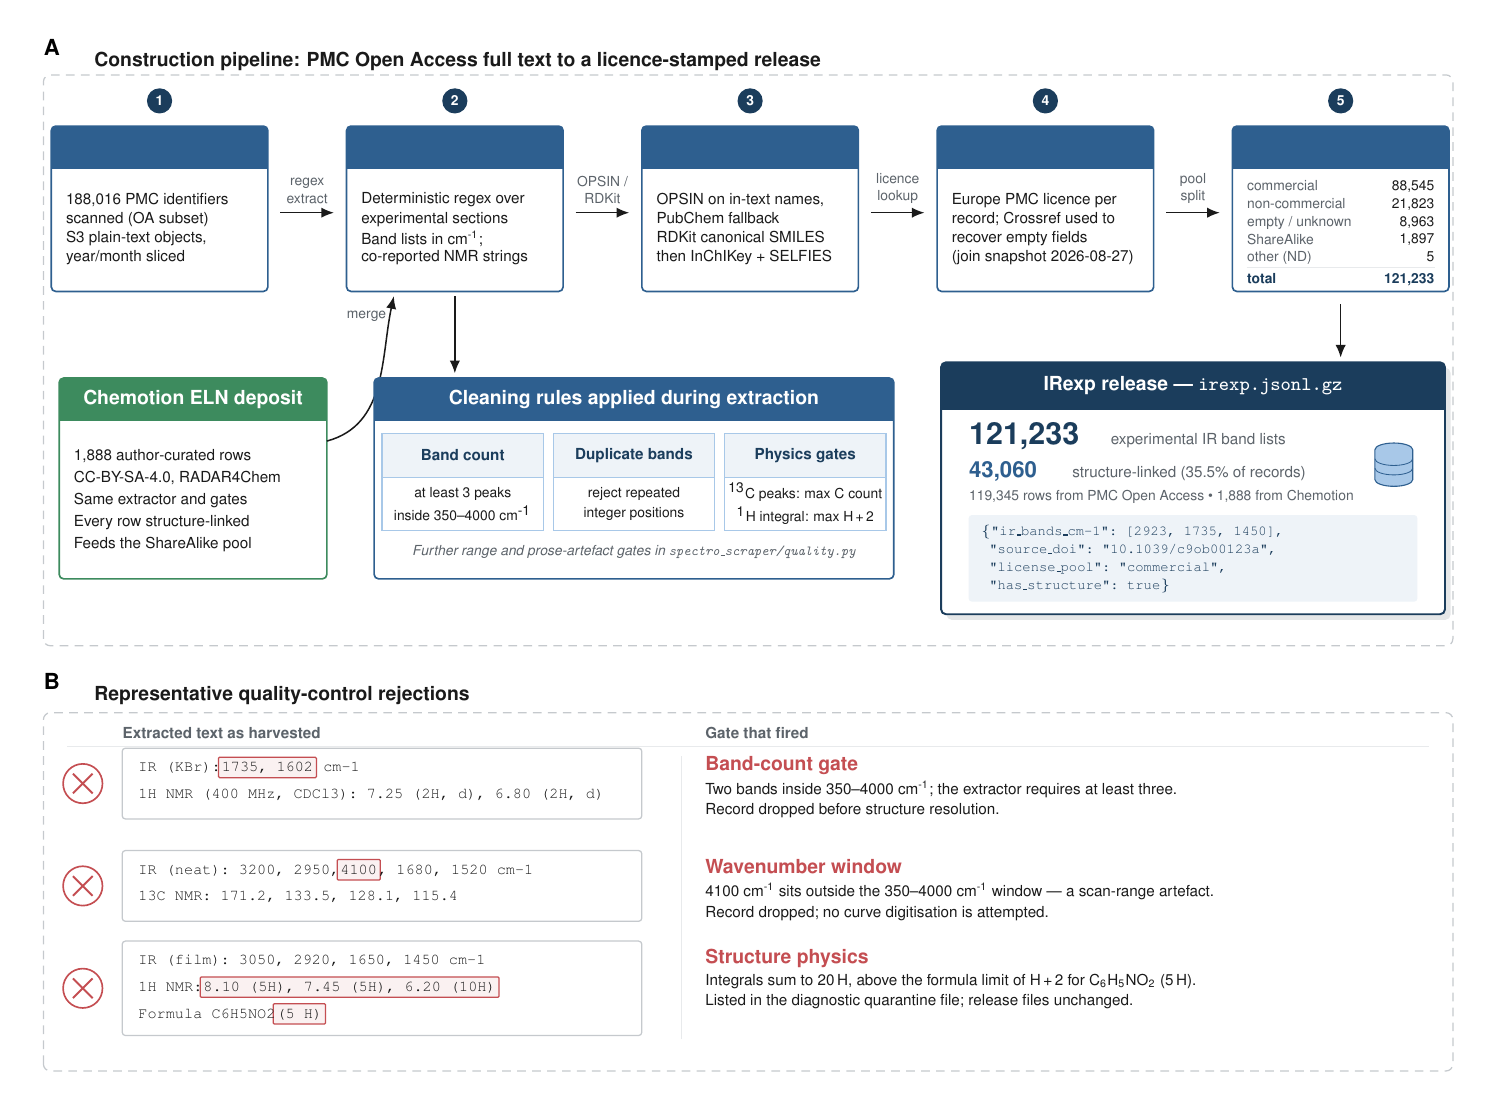
\begin{tikzpicture}[x=1mm,y=1mm,line cap=butt]
\useasboundingbox (0,1.5) rectangle (183,136.5);

% =====================================================================
%  PANEL A  --  construction pipeline
% =====================================================================
\node[anchor=north west,inner sep=0pt] at (2,135) {\PanelLabel{A}};
\node[anchor=base west,inner sep=0pt,text=ink,font=\FigBody] at (8.4,131.6)
  {\bfseries Construction pipeline: PMC Open Access full text to a licence-stamped release};
\draw[ghost,line width=0.45pt,rounded corners=2.5pt,dash pattern=on 1.1mm off 0.8mm]
  (2,58) rectangle (181,130.5);

% --- five stage cards ------------------------------------------------
\StageCard{3}{PMC OA full text}
\StepBadge{16.75}{1}
\CardLine{3}{0}{188,016 PMC identifiers}
\CardLine{3}{1}{scanned (OA subset)}
\CardLine{3}{2}{S3 plain-text objects,}
\CardLine{3}{3}{year/month sliced}

\StageCard{40.5}{IR extraction}
\StepBadge{54.25}{2}
\CardLine{40.5}{0}{Deterministic regex over}
\CardLine{40.5}{1}{experimental sections}
\CardLine{40.5}{2}{Band lists in cm\textsuperscript{-1};}
\CardLine{40.5}{3}{co-reported NMR strings}

\StageCard{78}{Structure resolution}
\StepBadge{91.75}{3}
\CardLine{78}{0}{OPSIN on in-text names,}
\CardLine{78}{1}{PubChem fallback}
\CardLine{78}{2}{RDKit canonical SMILES}
\CardLine{78}{3}{then InChIKey + SELFIES}

\StageCard{115.5}{Licence join}
\StepBadge{129.25}{4}
\CardLine{115.5}{0}{Europe PMC licence per}
\CardLine{115.5}{1}{record; Crossref used to}
\CardLine{115.5}{2}{recover empty fields}
\CardLine{115.5}{3}{(join snapshot 2026-08-27)}

\StageCard{153}{Release pools}
\StepBadge{166.75}{5}
\CardKV{153}{0}{commercial}{88,545}
\CardKV{153}{1}{non-commercial}{21,823}
\CardKV{153}{2}{empty / unknown}{8,963}
\CardKV{153}{3}{ShareAlike}{1,897}
\CardKV{153}{4}{other (ND)}{5}
\draw[faint,line width=0.35pt] (154.8,106.0) -- (178.7,106.0);
\node[anchor=north west,inner sep=0pt,text=nmrNavy,font=\FigTiny] at (154.8,105.4)
  {\bfseries total};
\node[anchor=north east,inner sep=0pt,text=nmrNavy,font=\FigTiny] at (178.7,105.4)
  {\bfseries 121,233};

% --- left-to-right connectors ---------------------------------------
\newcommand{\FlowArrow}[3]{%
  \draw[nature arrow] ({#1+1.6},\ArrowY) -- ({#1+\CardGap-1.6},\ArrowY);
  \node[anchor=south,align=center,inner sep=0pt,text=note,font=\FigTiny]
    at ({#1+\CardGap/2},{\ArrowY+1.1}) {#2\\[0.1ex]#3};%
}
\FlowArrow{30.5}{regex}{extract}
\FlowArrow{68}{OPSIN /}{RDKit}
\FlowArrow{105.5}{licence}{lookup}
\FlowArrow{143}{pool}{split}

% --- Chemotion branch, set to the same band as the gate inset --------
\begin{scope}
  \fill[white,rounded corners=1.6pt] (4,66.5) rectangle (38,92);
  \begin{scope}\clip[rounded corners=1.6pt] (4,66.5) rectangle (38,92);
    \fill[nmrGreen] (4,86.5) rectangle (38,92);
  \end{scope}
  \draw[nmrGreen,line width=0.6pt,rounded corners=1.6pt] (4,66.5) rectangle (38,92);
  \node[anchor=center,inner sep=0pt,text=white,font=\FigBody] at (21,89.25)
    {\bfseries Chemotion ELN deposit};
\end{scope}
\foreach \i/\t in {%
    0/{1,888 author-curated rows},
    1/{CC-BY-SA-4.0, RADAR4Chem},
    2/{Same extractor and gates},
    3/{Every row structure-linked},
    4/{Feeds the ShareAlike pool}}{%
  \node[anchor=north west,inner sep=0pt,text=ink,font=\FigSmall]
    at (5.8,{83.05-\i*2.8}) {\t};}
\draw[nature arrow] (38,84) to[out=15,in=258] (46.5,102.4);
% Set against the near-vertical head of the Bezier, not midway between it
% and the downward gate arrow, so the label cannot be read as either.
\node[anchor=east,inner sep=0pt,text=note,font=\FigTiny] at (45.6,99.8) {merge};

% --- quality-gate inset ---------------------------------------------
\draw[nature arrow] (54.25,102.4) -- (54.25,92.6);
\begin{scope}
  \fill[white,rounded corners=1.6pt] (44,66.5) rectangle (110,92);
  \begin{scope}\clip[rounded corners=1.6pt] (44,66.5) rectangle (110,92);
    \fill[nmrBlueDark] (44,86.5) rectangle (110,92);
  \end{scope}
  \draw[nmrBlueDark,line width=0.6pt,rounded corners=1.6pt] (44,66.5) rectangle (110,92);
  \node[anchor=center,inner sep=0pt,text=white,font=\FigBody] at (77,89.25)
    {\bfseries Cleaning rules applied during extraction};
\end{scope}
% three rule columns: header cell over a body cell, sharing one frame
\newcommand{\RuleCol}[4]{%
  \fill[tintBlue] (#1,79.4) rectangle ({#1+20.5},85);
  \draw[nmrBlueLight,line width=0.4pt] (#1,72.6) rectangle ({#1+20.5},85);
  \draw[nmrBlueLight,line width=0.4pt] (#1,79.4) -- ({#1+20.5},79.4);
  \node[anchor=center,inner sep=0pt,text=nmrNavy,font=\FigSmall] at ({#1+10.25},82.2)
    {\bfseries #2};
  \node[anchor=center,align=center,inner sep=0pt,text=ink,font=\FigTiny]
    at ({#1+10.25},76.0) {#3\\[0.35ex]#4};%
}
\RuleCol{45}{Band count}{at least 3 peaks}{inside 350--4000 cm\textsuperscript{-1}}
\RuleCol{66.75}{Duplicate bands}{reject repeated}{integer positions}
\RuleCol{88.5}{Physics gates}{\textsuperscript{13}C peaks: max C count}{\textsuperscript{1}H integral: max H\,+\,2}
\node[anchor=north,inner sep=0pt,text=note,font=\FigTiny] at (77,70.8)
  {\itshape Further range and prose-artefact gates in \texttt{spectro\_scraper/quality.py}};

% --- final release box ----------------------------------------------
\draw[nature arrow] (166.75,101.4) to[out=270,in=90] (166.75,94.6);
\begin{scope}
  \fill[ghost!45!white,rounded corners=1.8pt] (116.7,61.3) rectangle (180.7,93.3);
  \fill[white,rounded corners=1.8pt] (116,62) rectangle (180,94);
  \begin{scope}\clip[rounded corners=1.8pt] (116,62) rectangle (180,94);
    \fill[nmrNavy] (116,88) rectangle (180,94);
  \end{scope}
  \draw[nmrNavy,line width=0.7pt,rounded corners=1.8pt] (116,62) rectangle (180,94);
  \node[anchor=center,inner sep=0pt,text=white,font=\FigBody] at (148,91)
    {\bfseries IRexp release --- \texttt{irexp.jsonl.gz}};
\end{scope}
\node[anchor=base west,inner sep=0pt,text=nmrNavy,font=\NatureFont] at (119.5,83.6)
  {\fontsize{11}{11}\selectfont\bfseries 121,233};
\node[anchor=base west,inner sep=0pt,text=note,font=\FigSmall] at (137.5,83.6)
  {experimental IR band lists};
\node[anchor=base west,inner sep=0pt,text=nmrBlueDark,font=\NatureFont] at (119.5,79.4)
  {\fontsize{8}{8}\selectfont\bfseries 43,060};
\node[anchor=base west,inner sep=0pt,text=note,font=\FigSmall] at (132.6,79.4)
  {structure-linked (35.5\% of records)};
\node[anchor=base west,inner sep=0pt,text=note,font=\FigTiny] at (119.5,76.4)
  {119,345 rows from PMC Open Access \textbullet\ 1,888 from Chemotion};
\DbIcon{173.5}{81.0}
\fill[tintBlue,rounded corners=1.2pt] (119.5,63.6) rectangle (176.5,74.6);
\node[monoS,text=nmrNavy] (j1) at (121,72.0) {\{"ir\_bands\_cm-1":~[2923,~1735,~1450],};
\node[monoS,text=nmrNavy] (j2) at (121,69.7) {~"source\_doi":~"10.1039/c9ob00123a",};
\node[monoS,text=nmrNavy] (j3) at (121,67.4) {~"license\_pool":~"commercial",};
\node[monoS,text=nmrNavy] (j4) at (121,65.1) {~"has\_structure":~true\}};

% =====================================================================
%  PANEL B  --  QC rejections
% =====================================================================
\node[anchor=north west,inner sep=0pt] at (2,54.5) {\PanelLabel{B}};
\node[anchor=base west,inner sep=0pt,text=ink,font=\FigBody] at (8.4,51.1)
  {\bfseries Representative quality-control rejections};
\draw[ghost,line width=0.45pt,rounded corners=2.5pt,dash pattern=on 1.1mm off 0.8mm]
  (2,4) rectangle (181,49.5);

\node[anchor=base west,inner sep=0pt,text=note,font=\FigSmall] at (12,46.2)
  {\bfseries Extracted text as harvested};
\node[anchor=base west,inner sep=0pt,text=note,font=\FigSmall] at (86,46.2)
  {\bfseries Gate that fired};
\draw[faint,line width=0.35pt] (5,45.2) -- (178,45.2);
\draw[faint,line width=0.35pt] (83,8) -- (83,44);

% reject glyph: {x}{y}
\newcommand{\Reject}[2]{%
  \draw[nmrRed,line width=0.6pt] (#1,#2) circle (2.5mm);
  \draw[nmrRed,line width=0.7pt] ({#1-1.25},{#2-1.25}) -- ({#1+1.25},{#2+1.25});
  \draw[nmrRed,line width=0.7pt] ({#1-1.25},{#2+1.25}) -- ({#1+1.25},{#2-1.25});%
}
% Red highlight over a chained mono node.  Drawn on the background layer
% so that the tint never covers the excerpt it marks.
\newcommand{\Hilite}[1]{%
  \begin{pgfonlayer}{background}
    \draw[nmrRed,line width=0.45pt,rounded corners=0.4pt,fill=nmrRed!8]
      ([xshift=-0.35mm,yshift=-0.75mm]#1.base west) rectangle
      ([xshift=0.35mm,yshift=1.85mm]#1.base east);
  \end{pgfonlayer}%
}
% reason block: {top y}{rule}{line 1}{line 2}
\newcommand{\Reason}[4]{%
  \node[anchor=north west,inner sep=0pt,text=nmrRed,font=\FigBody] at (86,#1) {\bfseries #2};
  \node[anchor=north west,inner sep=0pt,text=ink,font=\FigSmall,align=left,inner ysep=0pt]
    at (86,{#1-3.1}) {#3\\[0.3ex]#4};%
}

% --- row 1: band-count gate -----------------------------------------
\Reject{7}{40.5}
\begin{pgfonlayer}{background}
  \draw[ghost,line width=0.45pt,rounded corners=1.2pt,fill=white] (12,36) rectangle (78,45);
\end{pgfonlayer}
\node[mono] (a1) at (14,42) {IR~(KBr):~};
\node[mono] (a2) at (a1.base east) {1735,~1602};
\node[mono] (a3) at (a2.base east) {~cm-1};
\node[mono] (a4) at (14,38.6) {1H~NMR~(400~MHz,~CDCl3):~7.25~(2H,~d),~6.80~(2H,~d)};
\Hilite{a2}
\Reason{44}{Band-count gate}%
  {Two bands inside 350--4000 cm\textsuperscript{-1}; the extractor requires at least three.}%
  {Record dropped before structure resolution.}

% --- row 2: window gate ---------------------------------------------
\Reject{7}{27.5}
\begin{pgfonlayer}{background}
  \draw[ghost,line width=0.45pt,rounded corners=1.2pt,fill=white] (12,23) rectangle (78,32);
\end{pgfonlayer}
\node[mono] (b1) at (14,29) {IR~(neat):~3200,~2950,~};
\node[mono] (b2) at (b1.base east) {4100};
\node[mono] (b3) at (b2.base east) {,~1680,~1520~cm-1};
\node[mono] (b4) at (14,25.6) {13C~NMR:~171.2,~133.5,~128.1,~115.4};
\Hilite{b2}
\Reason{31}{Wavenumber window}%
  {4100 cm\textsuperscript{-1} sits outside the 350--4000 cm\textsuperscript{-1} window --- a scan-range artefact.}%
  {Record dropped; no curve digitisation is attempted.}

% --- row 3: structure-physics gate ----------------------------------
\Reject{7}{14.5}
\begin{pgfonlayer}{background}
  \draw[ghost,line width=0.45pt,rounded corners=1.2pt,fill=white] (12,8.5) rectangle (78,20.5);
\end{pgfonlayer}
\node[mono] (c1) at (14,17.5) {IR~(film):~3050,~2920,~1650,~1450~cm-1};
\node[mono] (c2) at (14,14.1) {1H~NMR:~};
\node[mono] (c3) at (c2.base east) {8.10~(5H),~7.45~(5H),~6.20~(10H)};
\node[mono] (c4) at (14,10.7) {Formula~C6H5NO2~};
\node[mono] (c5) at (c4.base east) {(5~H)};
\Hilite{c3}\Hilite{c5}
\Reason{19.5}{Structure physics}%
  {Integrals sum to 20\,H, above the formula limit of H\,+\,2 for C\textsubscript{6}H\textsubscript{5}NO\textsubscript{2} (5\,H).}%
  {Listed in the diagnostic quarantine file; release files unchanged.}
\end{tikzpicture}
\end{document}
